

\section{Evaluation}
\label{sec:evaluation}

We plan to evaluate our method in two ways. Primarily, the methods ability to handle failure. To cope with the failure gracefully and cause the least amount of disturbance in the gameplay as possible. A secondary goal is to keep the latency of the game down as more clients and server are added to the system.

\subsection{Fault Tolerance}

The goal of the system was to gracefully cope with failing nodes without introducing latency. 
A game system design may choose to pause the processing of the game until the \gamestate becomes consistent again, during this time the players must wait for the game state to synchronize.
Game flow and minimal latency (as seen from a player of the game) is prioritized for consistency in this project.
In order to reduce latency consistency is sacrificed. 
When a node fails it could take a short amount of time to detect this failure as an inactivity.
During this time the agent for that node still exists in the game but is immobile.

Overall the system works as desired for graceful fault tolerance.
When a node fails the agent exists in the \gamestate for every node for a short period (a few seconds) after which all data related to the agent is removed from the \gamestate.

\subsection{Scalability vs Consistency}

It is difficult to measure the consistency between each of the nodes. 
We would have to employ a large logging system that would take snap shots of the \gamestate at points in time. 
In order for these snapshots to be effective there would need to be additional time synchronization across the nodes for comparison. 
Instead the relative number of successful shots is used to measure consistency. 
A successful shot is one that is initiated by a client, forwarded to the client's local server and again forwarded to the proper server for validation. 
The shot is successful if the last server agrees with the result of the shot. 
The occurrence of successful shot implies that $3$ \gamestates where at least partial consistent.
We measure the scalability by increasing the number of nodes in the system and comparing the relative number of fire events that are successful. 
	\begin{figure}[ht]
	\centering
		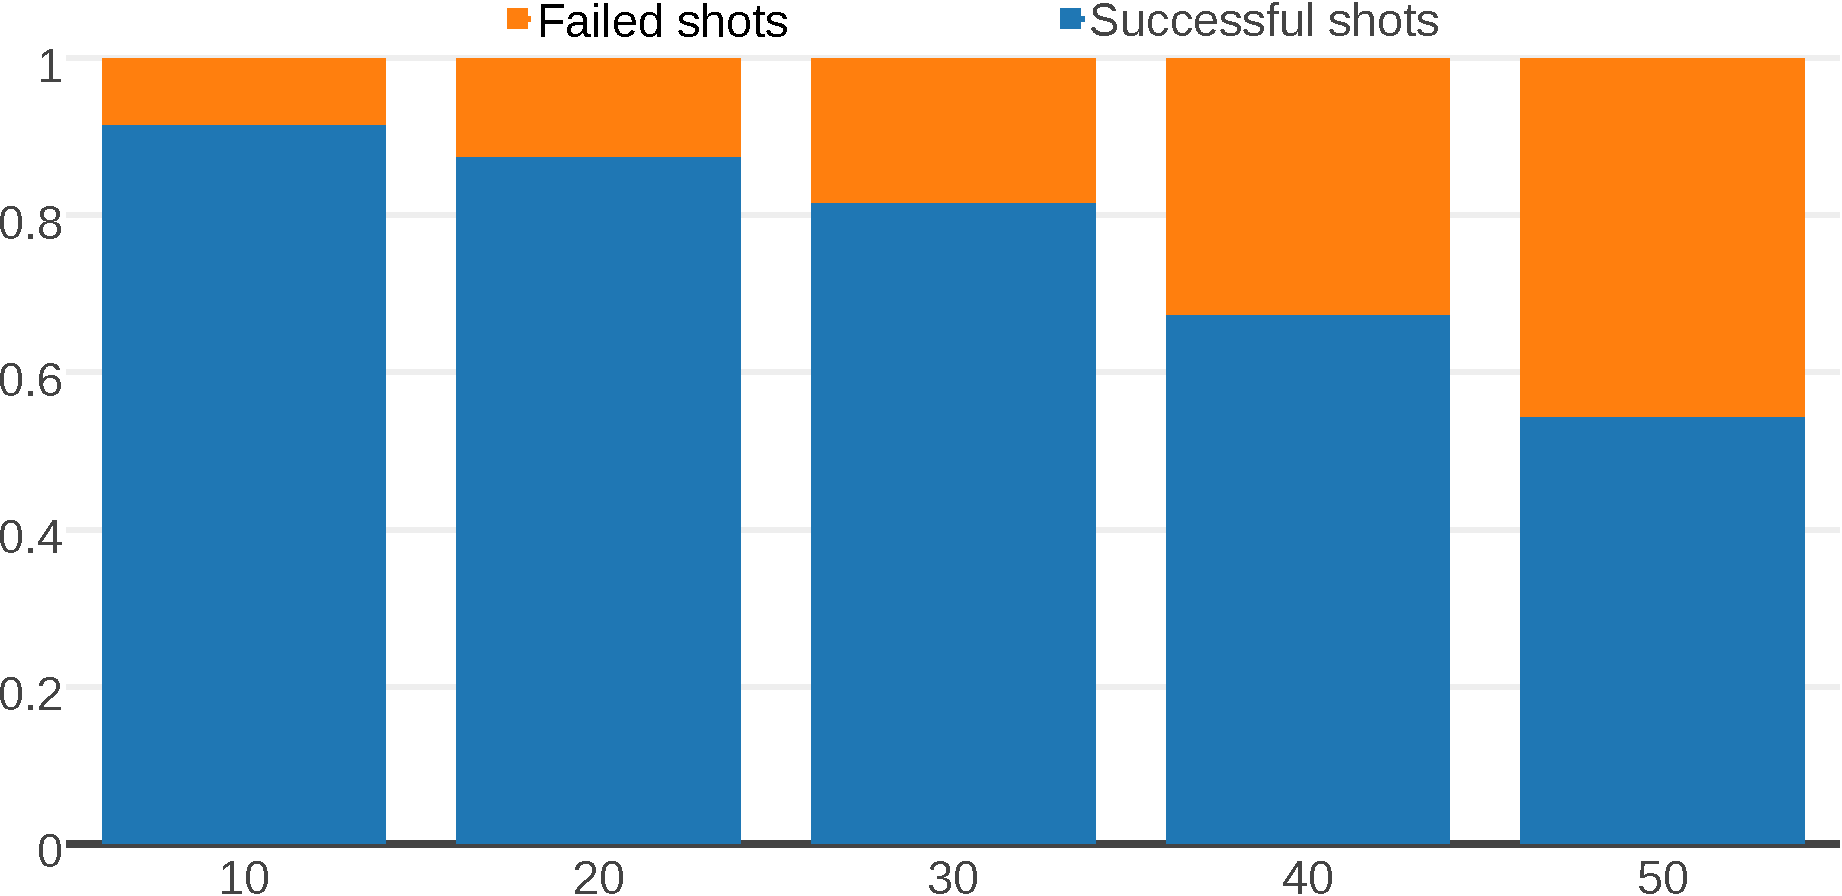
\includegraphics[width=0.95\linewidth]{../images/agents-vs-consistency-via-shots-crop.pdf}
		agents
		\caption{\label{figure:nodes-vs-shots-consistency} A chart of the relative numbers of successful shots vs failed shots. As the number of nodes in the system increases the relative number of successful shots decreases.}
	\end{figure}
Figure~\ref{figure:nodes-vs-shots-consistency} shows us how well the systems consistency copes with the number of nodes in the system. As expected, as the number of nodes increases the number of successful shots decreases. The decrease in successful shots is a proxy for the system consistency. 
This is the result of increased latency and dropped packets in the system. 

\subsection{Game Simulation}

Here a description of the game is given, along with some features of the client Artificial Intelligence. The game is confined to a 3D box of dimensions $10x10x10$. Inside the box all the agents are simulated using a pseudo randomized AI. A visualization of the \gamestate is shown in Figure~\ref{figure:game-renders}(a and b).

\begin{figure}[htb]
\centering
	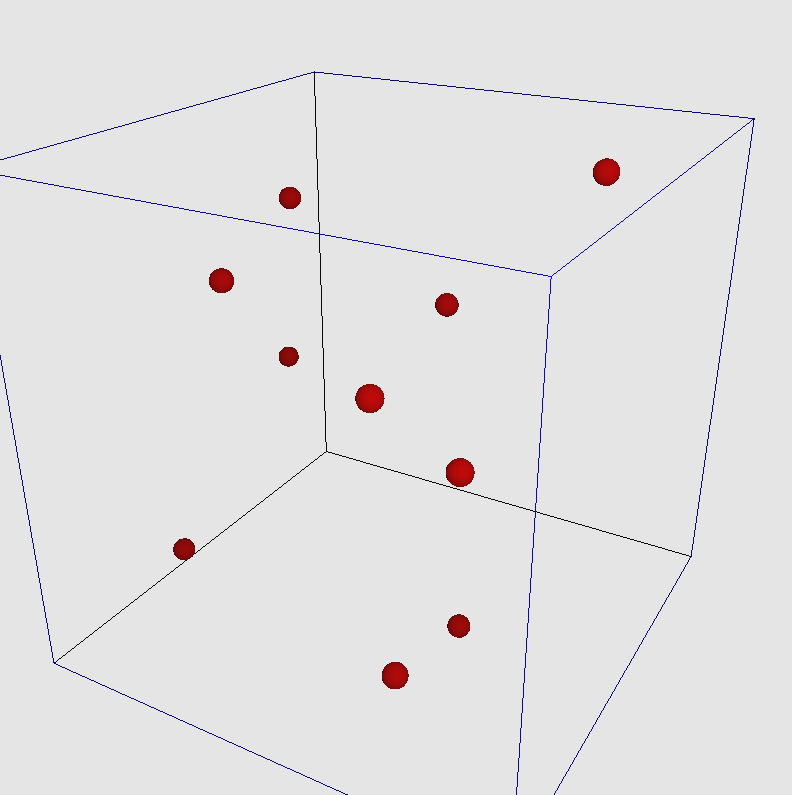
\includegraphics[width=0.45\linewidth]{../images/10-agents-render.png}
	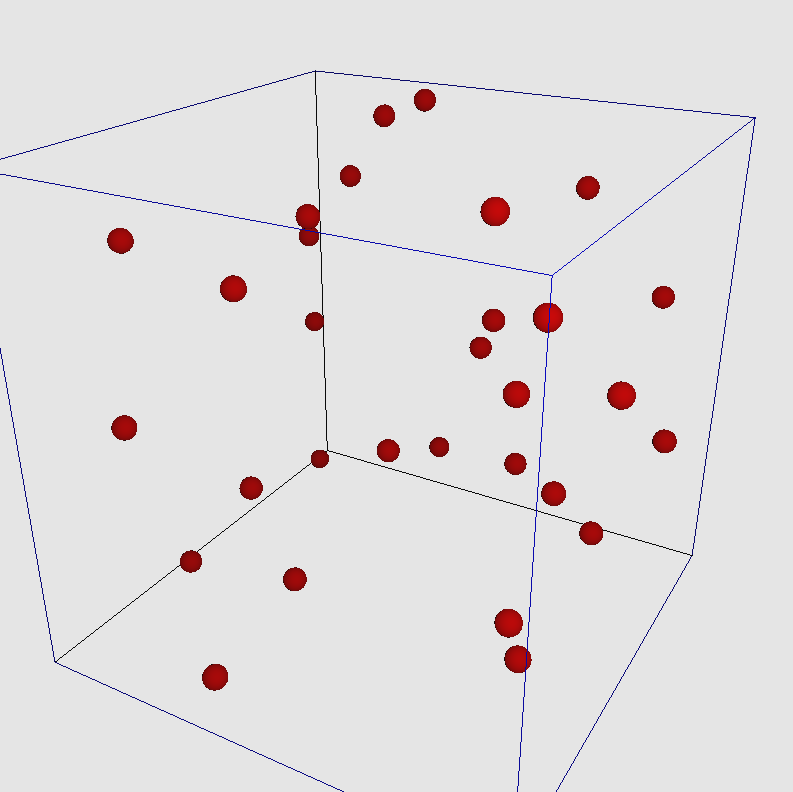
\includegraphics[width=0.45\linewidth]{../images/30-agents-render.png}	

	\caption{\label{figure:game-renders} Two rasterized simulation frames. On the left with $10$ agents and on the right with $30$ agents.}
\end{figure}

\noindent \textbf{RandomAI}: When an agent is initialized the agent is given a random starting position in the game. The agent is also given a random direction that the agent will travel. From this the agent will navigate along that direction of travel and bounce off the walls of the game box.

Each client will send an update of its location every $100ms$ and will update its own internal state every $100ms$ as well. The client can updated its state at faster intervals if desired. Each node will update its status in the \kvService every 2 seconds. The \activityServer will collect the node updates and post the updated list of active nodes every second. If a node dose not post an update for a duration of $6$ seconds, it is removed from the list of active nodes. In Table~\ref{table:gamestate-discription} the data a node stores to support the system is described. The \gamestate takes up the most amount of memory and it the most frequently updated structure.

\begin{table}[htb]
\centering
	\begin{tabular}{p{0.2\linewidth} | p{0.2\linewidth} | p{0.6\linewidth}}
	\textbf{Attribute name} & \textbf{Type} & \textbf{Description} \\ \hline
	\gamestate & map$<$string, Agent$>$ & map of agent identifiers to agent objects in the game \\ \hline
	Nodes & map$<$string, *net.UDPConn$>$ & map of nodes to the UDP connections to send messages to the nodes \\ \hline
	MyClientName & string  & identifier of the client this node is paired with\\  \hline
	ClientLink & *net.UDPAddr & UDP address of the client for this node\\ \hline
	Connection & *net.UDPConn & This nodes UDP listening connection \\ \hline	
	\end{tabular}
	\caption{\label{table:gamestate-discription} Layout of the data stored by each node.}
\end{table}
